\section{Event Selection}

Triggers selected for calibration are restricted to events where only a single pixel is hit by the cosmic muon.  This ensures the muon trajectory is nearly perpendicular and does not undergo multiple scattering.  As a result a uniform distribution of desposited MIP energy is seen by all the PMTs, which provides a more accurate calibration. An intitial skim was used to select events that are most likely to involve a single pixel hit, using a multiplicity cut and a geometrical constraint.

\FloatBarrier
\subsection{Multiplicity Cut}
The multiplicity cut removed any event that contained more than three PMT readouts (one from each layer). This reduces the number of cosmic ray events that are not perpendicular to the face of the PCAL unit.  If a cosmic ray trajectory is not perpendicular to the PCAL face, it can intercept multiple strips in one orientation (e.g. - strip U30 and U31 both receive a signal). Although the accepted range of non-perpendicular angles depends on the size of the strips and their overlapping shape, this effect is expect to average out.  This multiplicity cut also helps to remove events where multiple cosmic rays hit the detector within the same time interval.  Overall this cut removes 95\% of the triggered events. 

\FloatBarrier
\subsection{Dalitz Cut} 
The Dalitz cut relies on the geometry axiom that for any point inside an equilateral triangle, the sum of the distances to each edge of the triangle is constant.  The same result also applies to distances along the edge of the triangle, in which case the constant is equal to two.  Thus only PMT numbers are needed to test the Dalitz cut, rather than calculating the interior x and y coordinate for every hit.  Once the N=3 multiplicity cut is passed, only the Dalitz condition need be tested for the U,V,W combination of hit strips to ensure the combination arises from a single pixel. If this condition is not satisfied, then the hit recorded is most likely electronic noise, an indirect hit, or multiple cosmic ray hits recorded at once.

The relatively simple calculation is given by equations \ref{eq:udist}-\ref{eq:totaldist}.  The calculation uses normalized coordinates calculated from the number of the triggered PMTs, which compensates for the PCAL not being an equilateral triangle.  Examination of Figure \ref{fig:dalitz}~(left) shows that the N=3 multiplicity skim overwhelmingly favors events that produce a pixel, as indicated by the sharp peak at uvw=2 which contains most of the events.  An example of the kind of hit pattern that would cause events outside of the uvw=2 peak is shown in Figure \ref{fig:dalitz}~(right).

\begin{equation}
    dist(u) = \left\{
        \begin{array}{l l}
            u/84.0                       & \quad \text{if $u < 52$}\\
            (52.0 + (u - 52.0)\times2.0)/84.0 & \quad \text{if $u \geq 52$}
        \end{array} \right.{}
         \label{eq:udist}
\end{equation}

\begin{equation}
    dist(v) = \left\{
        \begin{array}{l l}
            2.0 \times v/77.0;                       & \quad \text{if $v < 15$}\\
            (30.0 + (v - 15.0))/77.0                 & \quad \text{if $v \geq 15$}
        \end{array} \right.{}
         \label{eq:vdist}
\end{equation}


\begin{equation}
    dist(w) = \left\{
        \begin{array}{l l}
            2.0 \times w/77.0;                       & \quad \text{if $w < 15$}\\
            (30.0 + (w - 15.0))/77.0                 & \quad \text{if $w \geq 15$}
        \end{array} \right.{}
         \label{eq:wdist}
\end{equation}


\begin{equation} 
    uvw = dist(u) +  dist(v) + dist(w)
    \label{eq:totaldist}
\end{equation}

\begin{figure}[h]
    \centering
    \begin{subfigure}[h]{0.44\textwidth}
        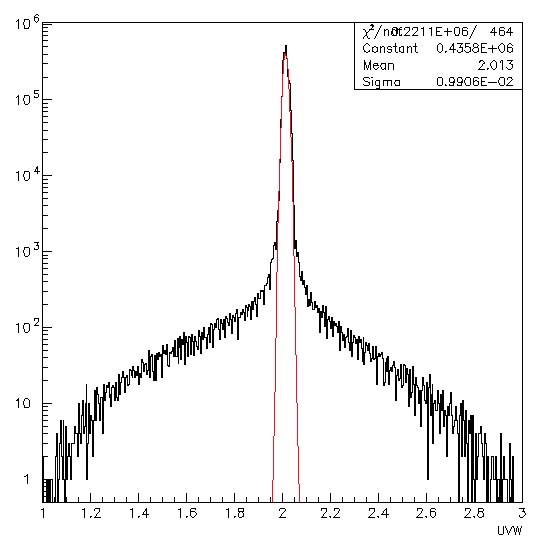
\includegraphics[height= 3in, keepaspectratio = true]{dalitz2}
        \label{fig:dalitz1}
    \end{subfigure}
    \begin{subfigure}[h]{0.55\textwidth}
        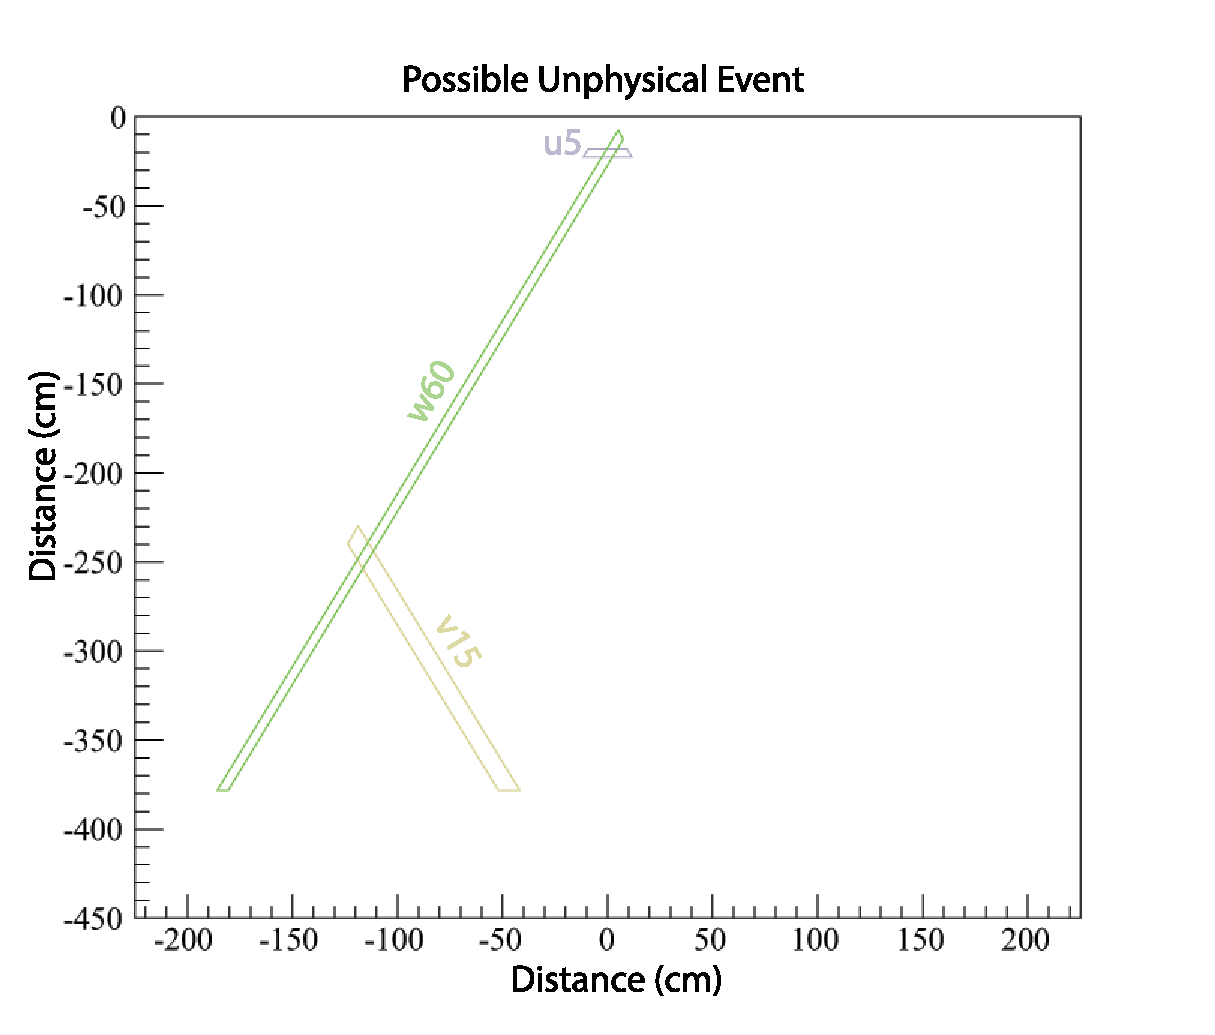
\includegraphics[height=3in, keepaspectratio = true]{unphysical}
        \label{fig:dalitz2}
    \end{subfigure}
\caption{LEFT: Histogram of Dalitz condition (\ref{eq:totaldist}) after multiplicity (N=3) skim of cosmic triggered data.\\ RIGHT: Example of an event that passed the N=3 cut, but fell outside of the Dalitz peak at uvw=2.}
\label{fig:dalitz}
\end{figure} 
\FloatBarrier
